\vspace{-0.5cm}
\textbf{Claim:} GNN can solve percolation problem $\implies$ GNN can solve connection problem\hfill
\newline
\begin{columns}[T]
    \begin{column}{0.7\textwidth}
        \textbf{Procedure:}
        \begin{enumerate}
            \item Start with arbitrary Graph $G$, select two nodes $n$, $m$
            \item Place $G$ inside unit square, move $n,m$ to edges, add edge ($n,m$) $\implies$ new graph $\tilde{G}$
            \item Run GNN on $\tilde{G}$
            \item $\tilde{G}$ percolating $\iff$ $n,m$ connected in $G$ 
        \end{enumerate}        
    \end{column}    
    \begin{column}{0.3\textwidth}
        \begin{figure}
        \begin{subfigure}[]{\textwidth}
            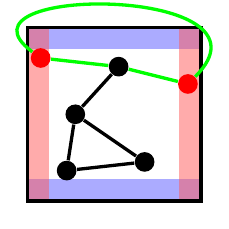
\begin{tikzpicture}[
                node/.style={circle, inner sep=0pt, fill=black, minimum size=2.5mm},
                node_c/.style={circle, inner sep=0pt, fill=red, minimum size=2.5mm}
            ]
            \useasboundingbox[fill=white](0,0) rectangle(0.55*4,0.55*4);
            \fill[blue!65, fill opacity=0.5] (0,0) rectangle (0.55*4, 0.55*0.5);
            \fill[blue!65, fill opacity=0.5] (0,0.55*3.5) rectangle (0.55*4, 0.55*4);
            \fill[red!65, fill opacity=0.5] (0,0) rectangle (0.55*0.5, 0.55*4);
            \fill[red!65, fill opacity=0.5] (0.55*3.5,0) rectangle (0.55*4, 0.55*4);
            \draw[black, very thick] (0,0) rectangle (0.55*4,0.55*4);
            \node[node_c] at (0.55*0.3, 0.55*3.3) (n1) {};
            \node[node] at (0.55*1.1, 0.55*2.0) (n2) {};
            \node[node] at (0.55*0.9, 0.55*0.7) (n3) {};
            \node[node] at (0.55*2.7, 0.55*0.9) (n4) {};
            \node[node] at (0.55*2.1, 0.55*3.1) (n5) {};
            \node[node_c] at (0.55*3.7, 0.55*2.7) (n6) {};
            \draw[very thick, green]  (n1) -- (n5);
            \draw[very thick]  (n5) -- (n2);
            \draw[very thick, green]  (n5) -- (n6);
            \draw[very thick]  (n2) -- (n4);
            \draw[very thick]  (n3) -- (n4);
            \draw[very thick]  (n2) -- (n3);
            \draw[very thick, green]  (n1) .. controls (-0.55*2,0.55*5) and (0.55*6,0.55*5) .. (n6);
            \end{tikzpicture} 
        \end{subfigure}
        \vskip0.5cm
        \begin{subfigure}[]{\textwidth}
            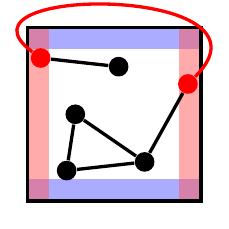
\begin{tikzpicture}[
                node/.style={circle, inner sep=0pt, fill=black, minimum size=2.5mm},
                node_c/.style={circle, inner sep=0pt, fill=red, minimum size=2.5mm}
            ]
            \useasboundingbox[fill=white](0,0) rectangle(0.55*4,0.55*4);
            \fill[blue!65, fill opacity=0.5] (0,0) rectangle (0.55*4, 0.55*0.5);
            \fill[blue!65, fill opacity=0.5] (0,0.55*3.5) rectangle (0.55*4, 0.55*4);
            \fill[red!65, fill opacity=0.5] (0,0) rectangle (0.55*0.5, 0.55*4);
            \fill[red!65, fill opacity=0.5] (0.55*3.5,0) rectangle (0.55*4, 0.55*4);
            \draw[black, very thick] (0,0) rectangle (0.55*4,0.55*4);
            \node[node_c] at (0.55*0.3, 0.55*3.3) (n1) {};
            \node[node] at (0.55*1.1, 0.55*2.0) (n2) {};
            \node[node] at (0.55*0.9, 0.55*0.7) (n3) {};
            \node[node] at (0.55*2.7, 0.55*0.9) (n4) {};
            \node[node] at (0.55*2.1, 0.55*3.1) (n5) {};
            \node[node_c] at (0.55*3.7, 0.55*2.7) (n6) {};
            \draw[very thick]  (n1) -- (n5);
            \draw[very thick]  (n2) -- (n4);
            \draw[very thick]  (n3) -- (n4);
            \draw[very thick]  (n2) -- (n3);
            \draw[very thick]  (n4) -- (n6);
            \draw[very thick, red]  (n1) .. controls (-0.55*2,0.55*5) and (0.55*6,0.55*5) .. (n6);
            \end{tikzpicture}   
        \end{subfigure}   
        \end{figure}
    \end{column}       
\end{columns}